\documentclass{article}

\usepackage[utf8]{inputenc}
\usepackage[T1]{fontenc}
\usepackage[greek,english]{babel}
\usepackage{alphabeta}
\usepackage{amsmath}
\usepackage{amssymb}
\usepackage{graphicx}
\usepackage{subcaption}
\usepackage{epstopdf}
\usepackage[margin=1in, paperwidth=7.5in,paperheight=10.5in]{geometry}
\usepackage{hyperref}
\usepackage{paracol}

\newcommand\course{ΗΡΥ 411}
\newcommand\courseName{Ενσωματωμένα Συστήματα Μικροεπεξεργατών}
\newcommand\semester{Χειμερινό 2020-2021}
\newcommand\assignmentNumber{Εργαστήριο 1}
\newcommand\studentName{Μαυρογιώργης Δημήτρης}                           
\newcommand\studentNumber{2016030016}

\title{\underline{\textbf{\assignmentNumber}}} 
\author{\textsc{\textbf{Όνομα:}}  \studentName\\
		\textsc{\textbf{ΑΜ:}}  \studentNumber\\
		\course \ - \courseName\\ 
		\textsc{Πολυτεχνείο Κρήτης}
		}
\date{\today}
\begin{document}
	\maketitle

\section*{Σκοπός}
	Σκοπός της πρώτης εργαστηριακής άσκησης είναι εξοικείωση με το περιβάλλον του Atmel Studio 7, στο οποίο γίνεται η ανάπτυξη μικροελεγκτών AVR. Πιο συγκεκριμένα, για την εξοικείωσή μας με το περιβάλλον ζητήθηκε να υλοποιήσουμε έναν χρονιστή διάρκειας 1 ms με δύο διαφορετικούς τρόπους: 1) με βρόγχο κατάλληλου αριθμού επαναλήψεων και 2) με τη χρήση timer/counter και interrupt του χρονιστή.
	
\section*{Υλοποίηση χρονιστή με βρόγχο επανάληψης}	
	Για τη συγκεκριμένη υλοποίηση του χρονιστή έπρεπε να υπολογίσουμε τον αριθμό των κύκλων που πρέπει να περιμένει ο χρονιστής έτσι, ώστε να έχουμε την επιθυμητή διάρκεια του 1 ms.
	Eιδικότερα, για συχνότητα ρολογιού 10 ΜHz, o αριθμός των κύκλων που πρέπει να περιμένει υπολογίζεται ως εξώς:
	
	$$cycles = \frac{f_{clk}}{f_{1ms}} = \frac{10^{7}}{10^{3}} = 10^{4} \ \ κυκλοι$$
	
	\noindent
	Επειδή, όμως οι καταχωρητές του μικροελεγκτή είναι των 8-bit, με το καταχωρητή-μετρητή μπορούμε να μετρήσουμε μέχρι το $2^8 - 1 = 255$. Γι' αυτό το λόγο θα χρειαστεί να χρησιμοποιήσουμε ένα διπλό loop, όπου στο εσωτερικό loop μετράμε απο 250 μέχρι το 0 και επαναλαμβάνουμε τις εντολές NOP, DEC και BRNE (συνολικά 4 κύκλοι), ενώ στο εξωτερικό από 10 μέχρι το 0.
	Οπότε με αυτό τον τρόπο επιτυγχάνουμε να καθυστερούμε για περίπου $250*4*10 = 10^4$ κύκλους, για την αρκίβεια λίγο παραπάνω από 10000 κύκλους (1 + (250 * 4 - 1 + 4) * 10 - 1 + 4 = 10034 κύκλοι). Για τον υπολογισμό του ακριβούς αριθμού των κύκλων αφαιρούμε 11 κύκλους, επειδή το BRNE στην τελευταία επανάληψη χρειάζεται 1 κύκλο. Tέλος, κατα τη διάρκεια αυτών των κύκλων εκτελέστηκαν οι εντολές LDI, NOP, BRNE, DEC και RET, οι οποίες συνολικά στο πλήθος είναι (1 + (250 * 3) + 3 ) * 10 + 1 = 7532 εντολές . \\

	\noindent
	\textbf{Επεξήγηση Κώδικα} \\
	\noindent
	Αρχικά, πρέπει να γίνει μία αρχικοποίηση του stack pointer στην αρχή της στοίβας, επειδή γίνεται κλήση συνάρτησης. Έπειτα, κάνουμε set το bit 0 του καταχωρητή DDRB, για να δηλώσουμε ότι το bit 0 του PORTB είναι έξοδος. Στη συνέχεια, κάνουμε clear το bit 0 του PORTB, ώστε να έχουμε αρχική κατάσταση του ακροδέκτη "0", και καλούμε τη ρουτίνα delay. Τέλος, μόλις επιστρέψει η ρουτίνα delay κάνουμε το bit 0 του PORTB "1" και καλόυμε πάλι στην delay, για να έχουμε την επιθυμητή καθυστέρηση του 1 ms. \\
	
	\noindent
	Τα συγκεκριμένα βήματα τα εκτελόυμε αενάως έτσι, ώστε να έχουμε εναλλαγή του ακροδέκτη από 0 σε 1 και το αντίστροφο. \\
	
	\noindent
	Τέλος, όσον αφορά την ρουτίνα delay, η ιδέα της υλοποίησης του διπλού βρόγχου επανάληψης, καθώς και οι εντολές που εκτελούνται κατα τη διάρκεια του 1 ms, αναλύθηκαν παραπάνω.\\	
		
	\begin{figure}[h!]
		\centering
		\begin{subfigure}[t]{0.5\textwidth}
			\centering
			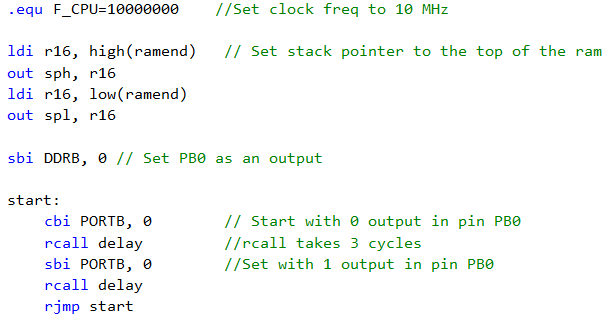
\includegraphics[width=0.8\linewidth]{./results/lab1a_init_main.png}
			\caption{Initialization of stack and registers and main program}
		\end{subfigure}%
		~
		\begin{subfigure}[t]{0.5\textwidth}
			\centering
			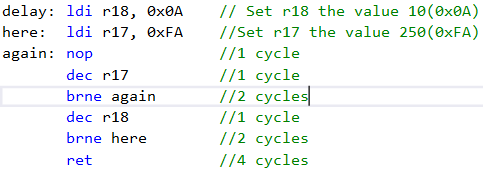
\includegraphics[width=\linewidth]{./results/lab1a_delay_code.png}
			\caption{Delay Subroutine for 1ms}
		\end{subfigure}
	\end{figure}
	
	\noindent
	\textbf{Προσομοίωση Αποτελεσμάτων} \\
	\noindent
	Στις δύο πρώτες εικόνες ( (a) και (b) ) παρατηρούμε ότι κατα τη διάρκεια του debugging ο καταχωρητης DDRB παίρνει τη σωστή τιμή 0x01, ενώ το bit 0 του PORTB που δηλώθηκε ως έξοδος αρχικοποιήθηκε με την τιμή "0" και παραμένει "0" για διάρκεια 1 ms. Μετά την κλίση της delay βλέπουμε οτι το bit 0 του PORTB αλλάζει από "0" σε "1" και κρατάει αυτή την τιμή για ακόμα 1 ms. \\
	Στις, επόμενες δύο εικόνες ( (c) και (d) ) παρατηρούμε ότι συμβαίνει το ακριβώς αντίθετο, δηλαδή το PORTB0 αλλάζει από από "1" σε "0" και και ξανά από "0" σε "1". Tέλος, από την επιλογή Stop Watch στο παράθυρο Processor Status βλέπουμε ότι η καθυστέρηση σε κάθε περίπτωση που περιγράφτηκε είναι η επιθυμητή του 1 ms περίπου.\\
	
	\begin{figure}[h!]
		\centering
		\begin{subfigure}[t]{0.5\textwidth}
			\centering
			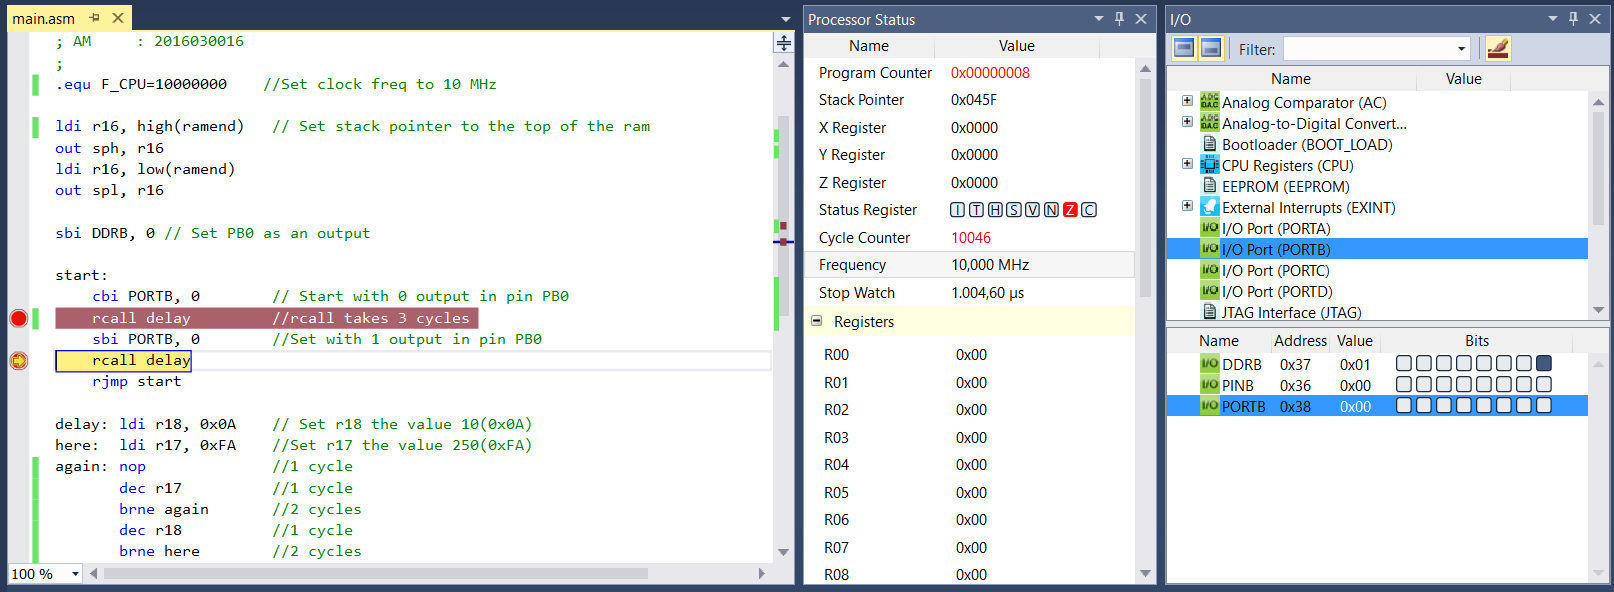
\includegraphics[width=\linewidth]{./results/lab1a_atmel_result_a.png}
			\caption{Results from Αtmel Studio 7 - PORTB0 is "0" for 1 ms}
		\end{subfigure}%
		~
		\begin{subfigure}[t]{0.5\textwidth}
			\centering
			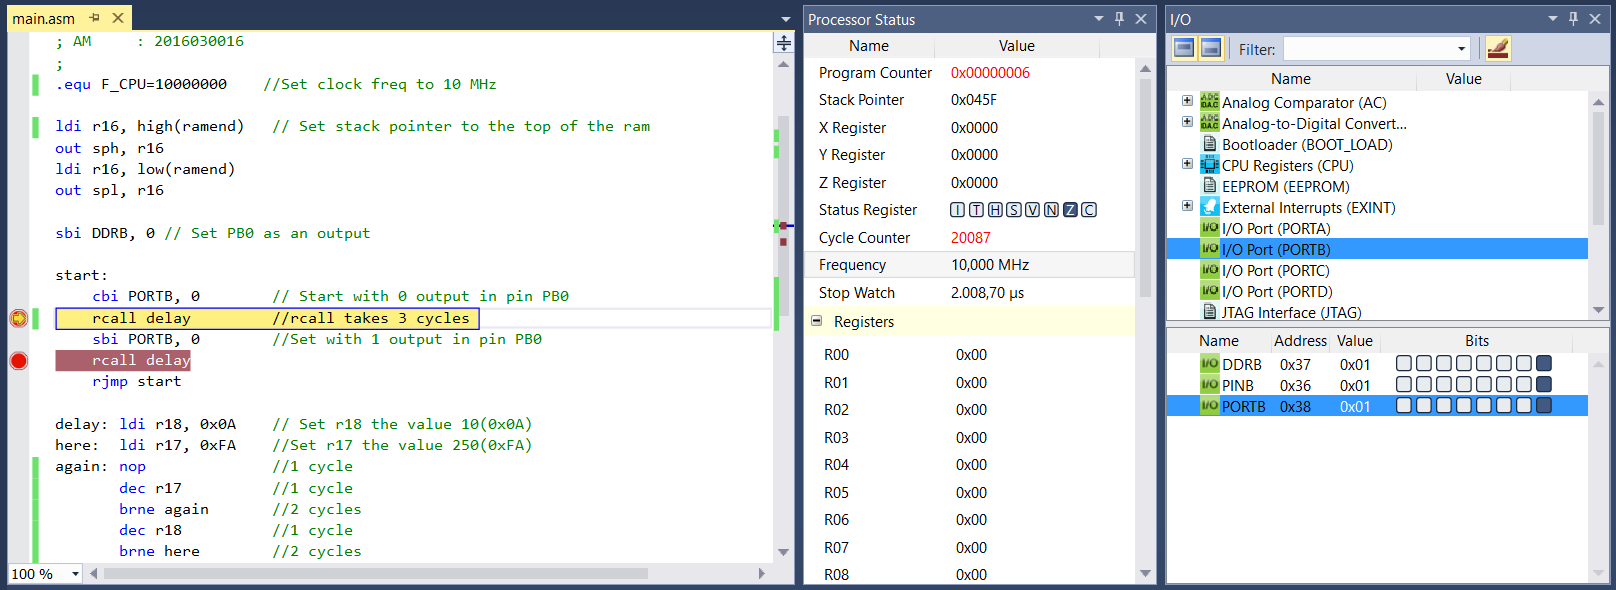
\includegraphics[width=\linewidth]{./results/lab1a_atmel_result_b.png}
			\caption{Results from Αtmel Studio 7 - PORTB0 changes from "0" to "1" and stays "1" for 1 ms}
		\end{subfigure}

		\begin{subfigure}[t]{0.5\textwidth}
			\centering
			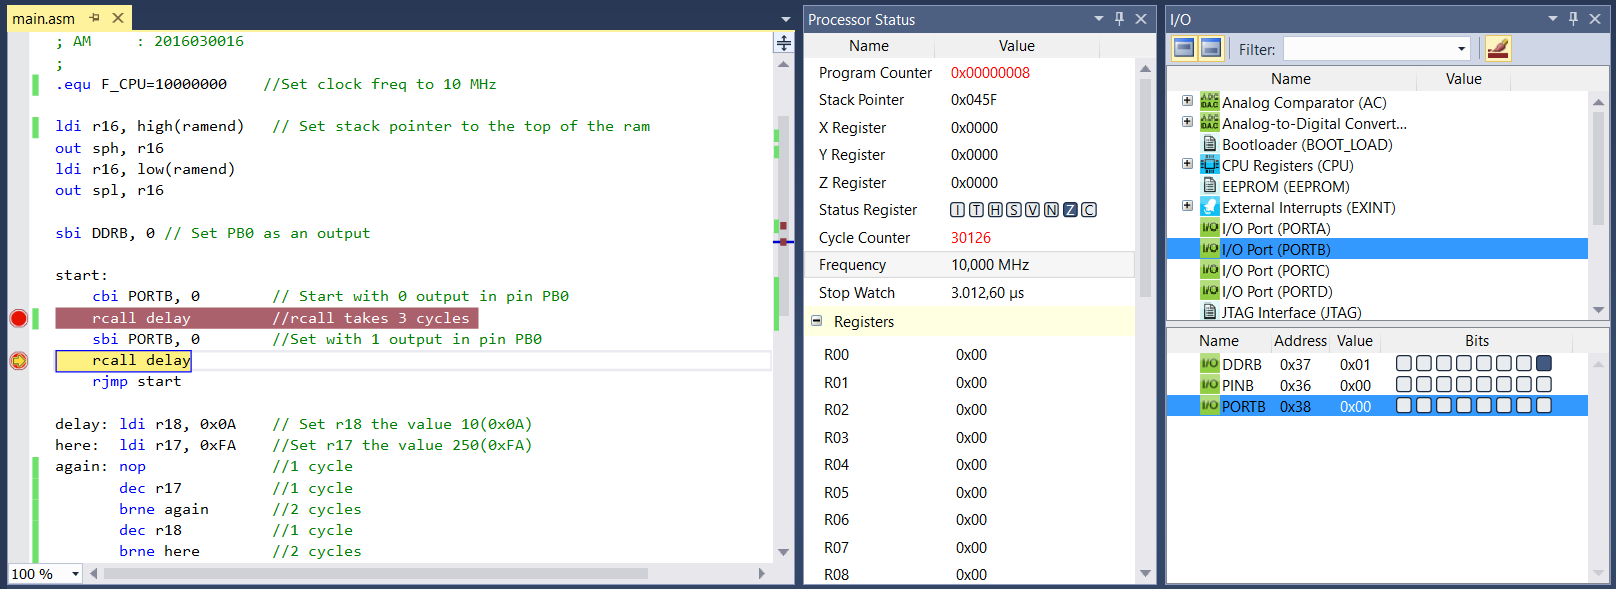
\includegraphics[width=\linewidth]{./results/lab1a_atmel_result_c.png}
			\caption{Results from Αtmel Studio 7 - PORTB0 changes from "1" to "0" and stays "0" for 1 ms}
		\end{subfigure}%
		~
		\begin{subfigure}[t]{0.5\textwidth}
			\centering
			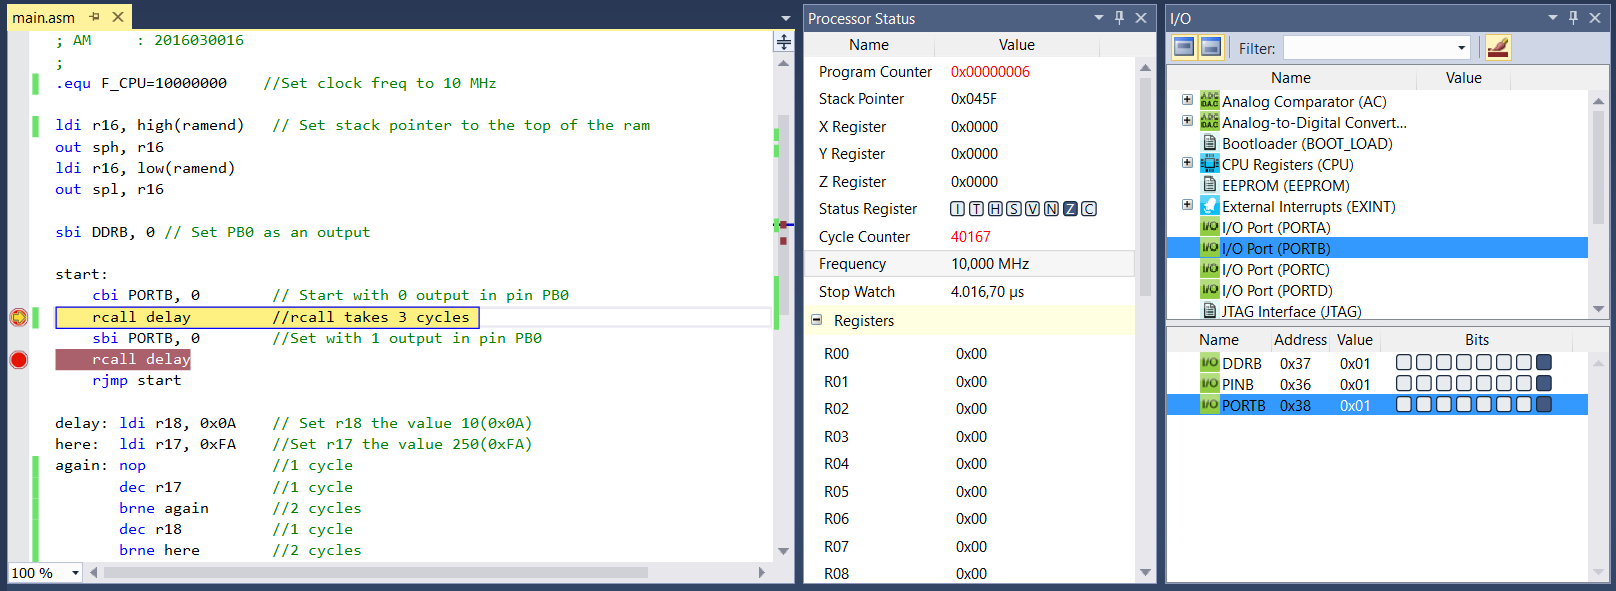
\includegraphics[width=\linewidth]{./results/lab1a_atmel_result_d.png}
			\caption{Results from Αtmel Studio 7 - PORTB0 changes from "0" to "1" and stays "1" for 1 ms}
		\end{subfigure}
	\end{figure}

\pagebreak
\section*{Υλοποίηση χρονιστή με τη χρήση timer/counter και interrupt}
Για την υλοποίηση του χρονιστή με τη χρήση του timer/counter0 και interrupt, χρειάστηκε να υπολογίσουμε την τιμή αρχικοποίησης των καταχωρητών TCNT0, TCCR0 και TIMSK.\\
Η τιμή αρχικοποίησης του καταχωρητή TCNT0 υπολογίστηκε ως εξής:
$$TCNT0\_VAL = MAX\_VAL - \frac{DELAY*FREQ}{PRESCALE} = 255 - \frac{1 ms * 10 MHz}{64} \approx 99 (0x063) $$

\noindent
Mετά από δοκιμές, η ελάχιστη τιμή του prescale που χρειαζόμαστε για να επιτύχουμε τη ζητούμενη καθυστέρηση είναι 64. Mε δεδομένο αυτό, θα πρέπει να θέσουμε τα 3 LSB (CS02, CS01 και CS00)του καταχωρητή TCCR0 με την τιμή "011". Επιπλέον, επειδή θελουμε ο μετρητής να μετρά από το 99 ως το 255, θα πρέπει να αρχικοποιήσουμε τα bit WGM00 και WGM01 με την τιμή "0", η οποία υποδηλώνει ότι ο μετρητής τρέχει σε normal mode, δηλαδή προς τα πάνω. Τέλος, όσον αφορά τον καταχωρητή TIMSK, θα πρέπει να θέσουμε το bit TOIE0 με την τιμή "1" έτσι, ώστε να ενεργοποιήσουμε τα interrupt του timer/counter0. Συνεπώς, με βάση την παραπάνω ανάλυση η τιμή αρχικοποίησης του TCNT0 είναι η "0x063", του TCCR0 έιναι η "0x03" και του TIMSK η "0x01".\\

\noindent
Κατα τη διάρκεια εκτέλεσης του προγράμματος και μέχρι να έρθει το Interrupt από τον timer/counter0, θα έχουν περάσει 157 * 64 = 10048 κύκλοι, καθώς ο μετρητής μετράει από το 99 μέχρι το 255 (157 φορές) και κάθε φορά που αυξάνεται κατά 1 περνάνε 64 κύκλοι του ρολογιού. Επιπλέον, μέσα σε αυτύς τους κύκλους εκτελούνται 1 εντολή NOP (1 cycle) και ένα RJMP (2 cycles). Συνεπώς, το συνολικό πλήθος των εντολών που εκτελούνται είναι 3350 NOP και 3349 RJMP, δηλαδή 6699 εντολές.\\

\noindent
\textbf{Επεξήγηση Κώδικα} \\
\noindent
Aρχικά, ορίζουμε με την εντολή .org τη διεύθυνση που ξεκινάει το πρόγραμμα και τη διεύθυνση του interrupt handler. Έπειτα, αφού κάνουμε τις αρχικοποιήσεις των καταχωρητών, όπως αναλύθηκε παραπάνω, θέτουμε το bit 0 του DDRB "1", για να δηλώσουμε ότι το PORTB0 είναι έξοδος, ένω το αρχικοποιούμε με "0". Tέλος, για ενεργοποιήσουμε τα global interrupt καλούμε την εντολή SEI, η οποία θέτει το I-bit του Status Register με "1".\\

\noindent
Όσον αφορά τον κύριο κορμό του προγράμματος, δηλαδή τη main, εκτελούμε εντολές NOP, μέχρι να έρθει το interrupt από τον timer/counter0 και να εκτελεστεί ο handler.\\

\noindent
Tἐλος, στον handler το μόνο που χρειάζεται να κάνουμε είναι να αλλάξουμε την τιμή της εξόδου PORTB0 και να αρχικοποιήσουμε πάλι τον καταχωρητή TCNT0 με την τιμή "0x63", ώστε να έχουμε σε κάθε κύκλο τη σωστή καθυστέρηση του 1 ms.

\begin{figure}[h!]
	\centering
	\begin{subfigure}[t]{0.5\textwidth}
		\centering
		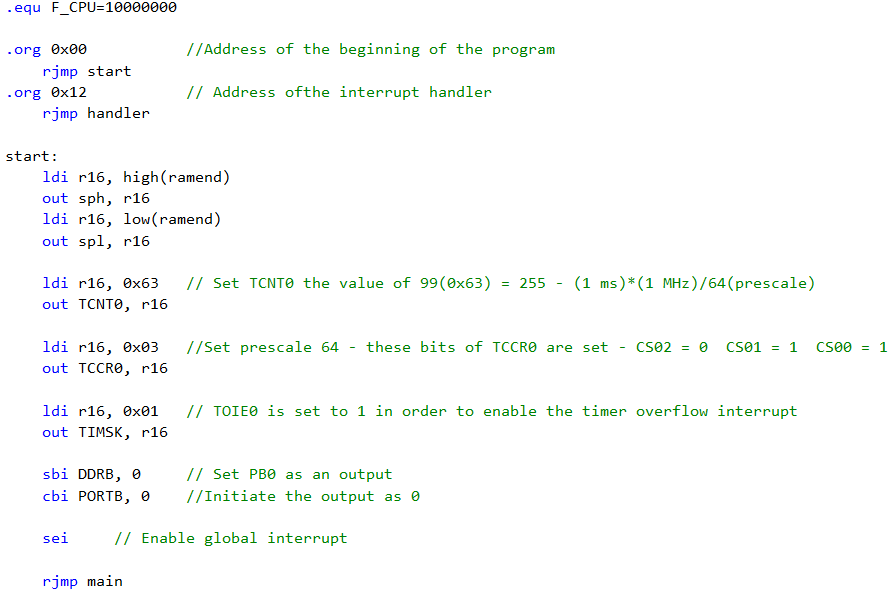
\includegraphics[width=0.6\linewidth]{./results/lab1b_init_code.png}
		\caption{Initialization of stack and registers}
	\end{subfigure}%
	~
	\begin{subfigure}[t]{0.5\textwidth}
		\centering
		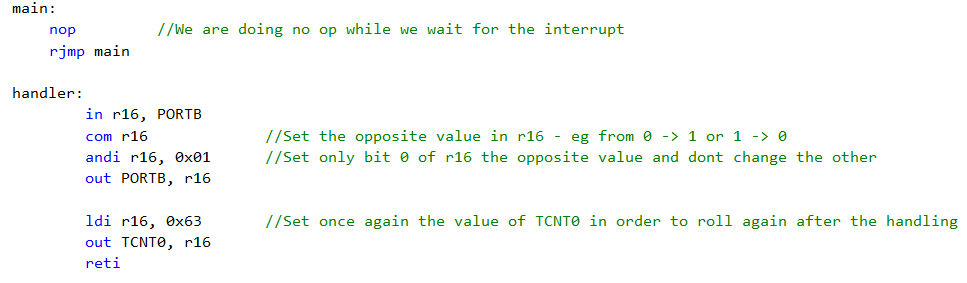
\includegraphics[width=\linewidth]{./results/lab1b_handler_code.png}
		\caption{Main program and interrupt handler}
	\end{subfigure}
\end{figure}

\pagebreak
\noindent
\textbf{Προσομοίωση Αποτελεσμάτων} \\
\noindent
Mε βάση τα παρακάτω αποτελέσματα προσομοίωσης, παρατηρούμε ότι o καταχωρητής DDRB έχει πάρει τη σωστή τιμή "0x01" και ότι το PORTB0 έχει αρχικοποιηθεί με "0". Παράλληλα, από τις εικόνες φαίνεται ότι και το I-bit του Status Register έχει πάρει την κατάλληλη τιμή "1", που σημαίνει ότι έχουν ενεργοποιηθεί τα global interrupts.\\

\noindent
Eπιπλέον, βλέπουμε ότι το PORTB0 έχει τιμή "0" για περίπου 1 ms, μέχρι που έρχεται το interrupt και εκτελείται ο handler, ο οποίος αλλάζει την τιμή του σε "1" (εικόνες (a) και (b)). Στις εικόνες (c) και (d), βλέπουμε ότι το PORTB0 παραμένει "1" για περίπου 1 ms, ενώ όταν έρχεται το interrupt η τιμή του γίνεται "0". Τέλος, όπως φαίνεται και στην εικόνα (ε), oι καταχωρητές TCNT0, TCCR0 και TIMSK έχουν αρχικοποιηθεί και αυτοί με τις σωστές τιμές που αναφέρθηκαν κατα την ανάλυση του προγράμματος. 
\begin{figure}[h!]
	\centering
	\begin{subfigure}[t]{0.5\textwidth}
		\centering
		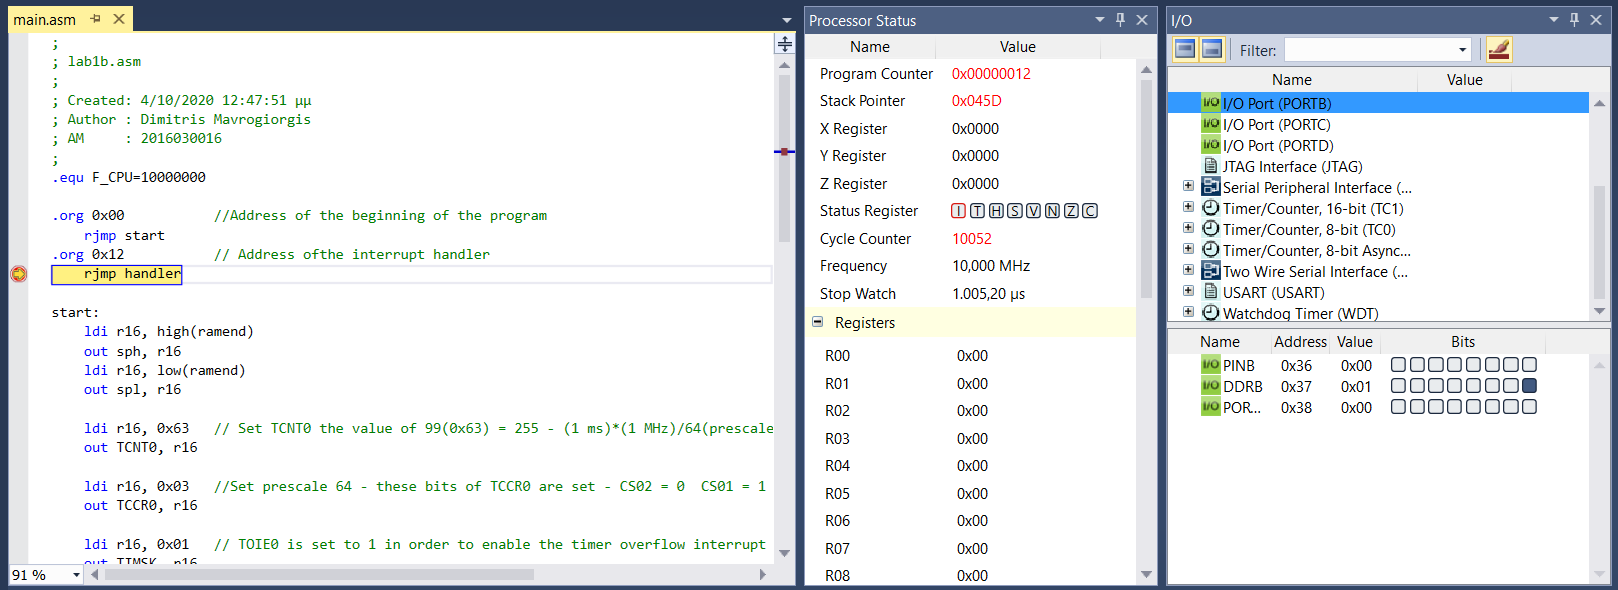
\includegraphics[width=\linewidth]{./results/lab1b_atmel_result_a.png}
		\caption{Results from Αtmel Studio 7 - PORTB0 is "0" for 1 ms}
	\end{subfigure}%
	~
	\begin{subfigure}[t]{0.5\textwidth}
		\centering
		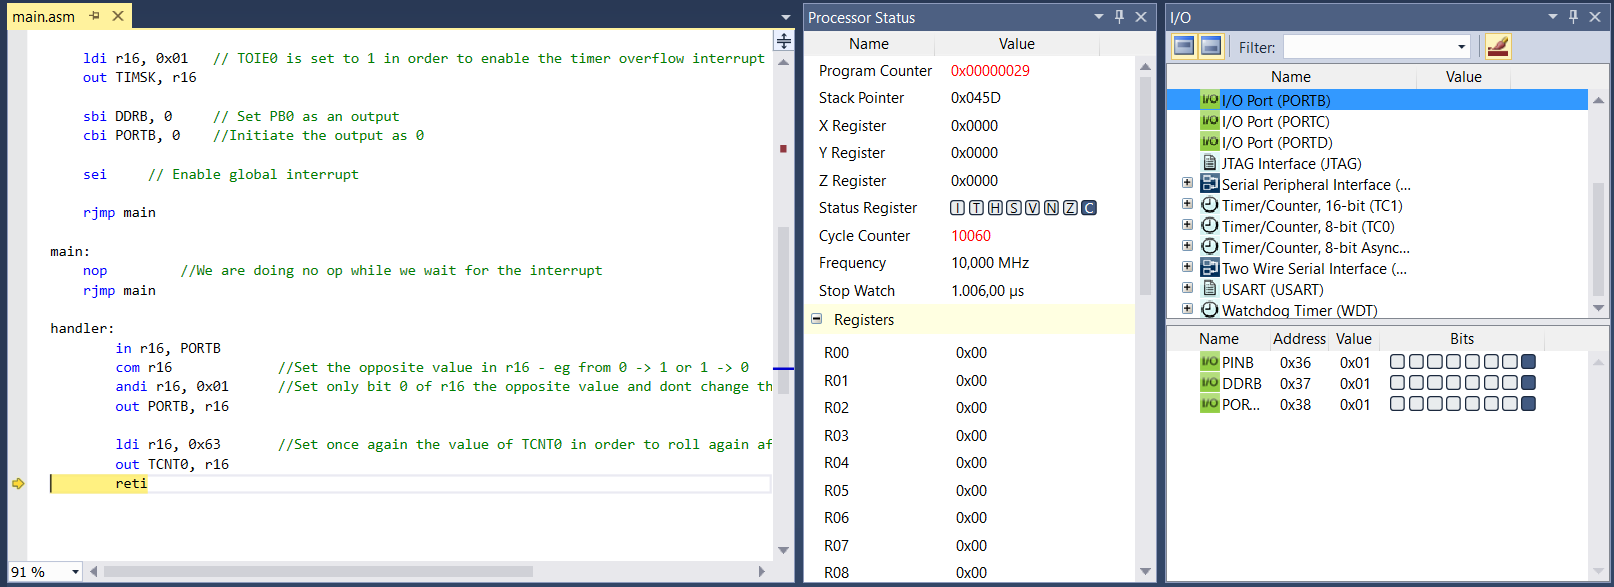
\includegraphics[width=\linewidth]{./results/lab1b_atmel_result_b.png}
		\caption{Results from Αtmel Studio 7 - Interrupt Handler Execution - PORTB0 changes from "0" to "1"}
	\end{subfigure}
	
	\begin{subfigure}[t]{0.5\textwidth}
		\centering
		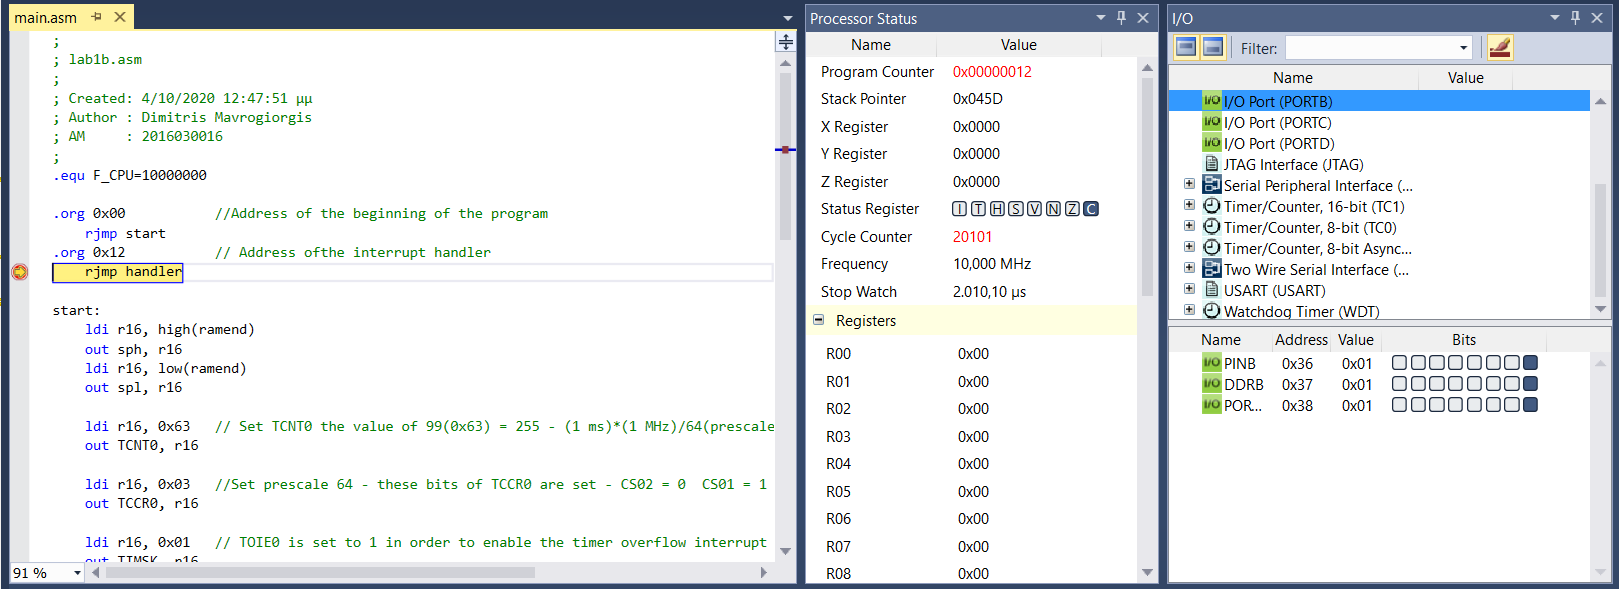
\includegraphics[width=\linewidth]{./results/lab1b_atmel_result_c.png}
		\caption{Results from Αtmel Studio 7 - PORTB0 is "1" for 1 ms}
	\end{subfigure}%
	~
	\begin{subfigure}[t]{0.5\textwidth}
		\centering
		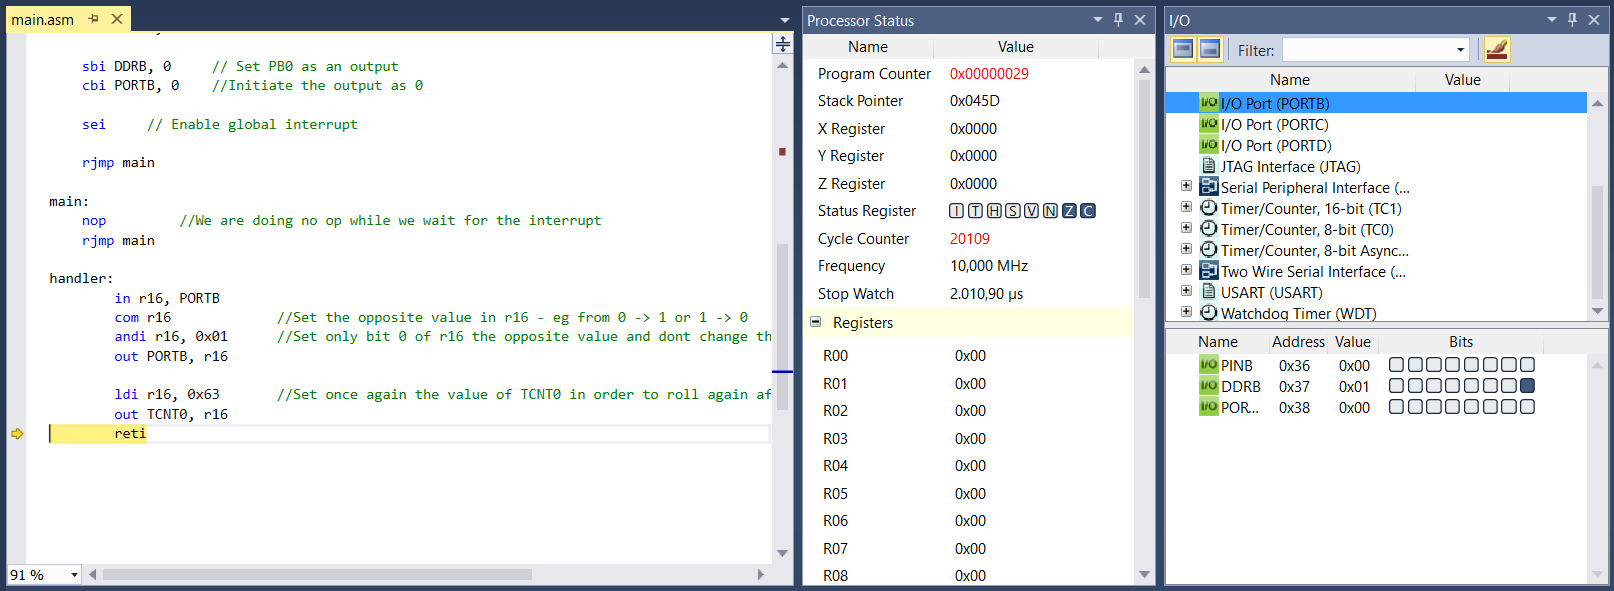
\includegraphics[width=\linewidth]{./results/lab1b_atmel_result_d.png}
		\caption{Results from Αtmel Studio 7 - Interrupt Handler Execution - PORTB0 changes from "1" to "0"}
	\end{subfigure}

	\begin{subfigure}[t]{0.5\textwidth}
		\centering
		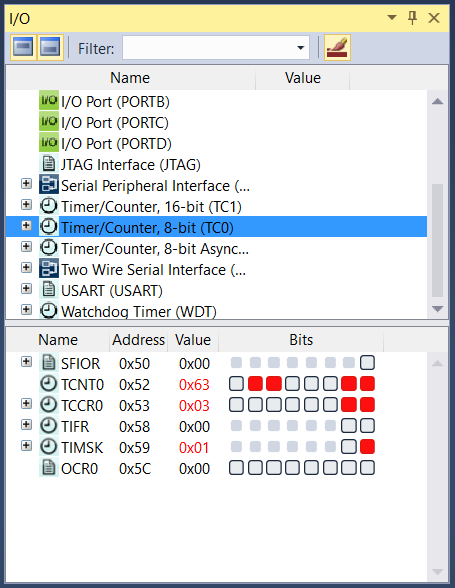
\includegraphics[width=0.5\linewidth]{./results/lab1b_reg_init.png}
		\caption{Results from Αtmel Studio 7 - Timer/Counter0 Register Initialization}
	\end{subfigure}
\end{figure}
\end{document}
